
\chapter{Mechanism of orientation selectivity in the tree shrew primary visual cortex}


\section{Summary}


\section{Introduction}

The tree shrew is a highly visual mammal that is closely related to
primates. While in the cat visual system, sharp orientation selectivity
is already present in layer 4 of the primary visual cortex, in macaques
and tree shrews, this transformation occurs from layer 4 to layer 2/3.
Similarly, where in the cats, LGN neurons are low pass tuned for spatial
frequency, layer 4 neurons show band-pass spatial frequency tuning, in
the tree shrews this transformation occurs from layer 4 to layer 2/3 in
V1. In this chapter, we examined if the orientation selectivity of the
tree shrew layer 2/3 neurons arise from a similar mechanism as has been
described in cats and macaques. As the sharpening of feature selectivity
occurs entirely within V1, experimenting in tree shrews gives us the
opportunity to examine the mechanism through which receptive field
properties are generated within a single electrode track rather than
paired recordings from more than one visual area. This also gives us the
added advantage of recording from neurons that are matched for
eccentricity, as this is an important caveat while comparing spatial
frequency tuning from different visual areas.

In the tree shrew, orientation selectivity in layer 2/3 neurons was
initially thought to have originated from excitatory convergence of a
number of layer 4 neurons arranged in a row (Mooser et al., 2004) as has
been proposed in cats and macaques (Hubel \& Wiesel, 1962; 1968).
However, when the data was carefully examined, it was found that the
elongation of the receptive fields in shrew layer 2/3 was much smaller
than would have been expected from a purely feed-forward mechanism. As a
result, it was proposed that the prominent horizontal connections
present in layer 2/3 further sharpened the orientation selectivity of
neurons (Bosking et al., 1997; Chisum et al., 2003; Mooser et al., 2004;
Veit et al., 2013). One study that used optogenetics and optical imaging
of intrinsic signals however showed that horizontal connections in the
layer 2/3 of tree shrew V1 did not have a modulatory effect on the
neuronal responses as previously suggested but rather had an additive
effect (Huang et al., 2014). Recently, Lee et al. (2016), suggested that
the orientation selectivity in the shrew V1 was established by the
spatially off on and off inputs as has been proposed in the cats (Soodak
\ldots{}Kremkow et al., 2016). However, Muly and Fitzpatrick (1992)
showed that on and off inputs to layer 2/3 cells have significant
overlap, preventing extensive segregation of sub-regions in tree shrews.
As a result, the mechanism through which orientation tuning comes about
in the shrew V1 is as yet unclear.

It is possible that orientation selectivity in the tree shrews can arise
from the anisotropic LGN Driven-Recurrent Model (ALD-RM; Vidyasagar et
al., 1996; Kuhlmann \& Vidyasagar, 2011; see Figure 1). In the cortex,
most cortical neurons receive direct excitatory inputs from sub-cortical
neurons biased for orientation and di-synaptic input from un-oriented
sub-cortical neurons via inhibitory interneurons (Creutzfeldt \& Ito,
1968; Ferster \& Lindstrom, 1983). The inhibitory input increases the
threshold for firing in the cortical neuron and the remaining signal
would automatically be tuned for orientation. Orientation selectivity
could then be further sharpened by intracortical mechanisms such as
recurrent excitation (Ref) and cross-orientation inhibition (ref). The
ALD-RM model also explained the spatial frequency tuning of neurons in
both the LGN as well as the layer 4 neurons in cats. LGN neurons showed
low-pass spatial frequency tuning (Ref) and at these spatial
frequencies, they fire well to all orientations (Vidyasagar \& Heide,
1984). At higher spatial frequencies however, the neurons show
orientation selectivity. Cortical neurons show band-pass spatial
frequency tuning and fire only at spatial frequencies where the LGN
neurons are tuned to orientation (Ref). The di-synaptic inhibition in
cortical neurons will be non-specific to orientation at lower spatial
frequencies where the LGN neuron is not tuned to orientation and causes
general attenuation at these lower spatial frequencies. At higher
spatial frequencies, the signal that remains is sharply tuned to both
the orientation and spatial frequency. The receptive fields of the
neurons in such a scheme in cat is shown in figure 1b.

\begin{figure}[H]
	\centering
	\includegraphics[width=0.8\linewidth]{ShrewV1/orituning_scheme.jpg}
	
	\caption{Mechanism of orientation selectivity proposed in cats and tree
		shrews. In the cats, layer 4 neurons receive excitatory input from an
		LGN neuron biased for the same orientation and di-synaptic input via an
		inhibitory neuron from an LGN neurons unbiased for orientation. The
		orientation non-specific inhibitory input increases the threshold of
		firing from the cortical neuron and the resulting signal is tuned for
		orientation. A similar transformation occurred from layer 4 to layer 2/3
		in the tree shrews.}
	\label{fig:orischeme}
\end{figure}



In figure 1b, the excitatory and inhibitory inputs to a layer 2/3 neuron
in the tree shrew cortex are shown. Each layer 2/3 neuron in the tree
shrew V1 receives converging excitatory inputs from on and off layer 4
neurons (Muly \& Fitzpatrick, 1992) and has extensive horizontal
connections (Bosking et al., 1997). Layer 4 neurons are also broadly
tuned to orientation and show low pass spatial frequency tuning while
layer 2/3 neurons show sharp orientation selectivity and show band-pass
spatial frequency tuning (Van Hooser et al., 2013). It could be that a
similar transformation that occurs from LGN to layer 4 in the cat visual
system happens from layer 4 to layer 2/3 in the tree shrews. We tested
the following hypothesis to test whether this was indeed the case.

\textbf{(H1)} As neurons in the on and off sub-divisions of layer 4
converge onto layer 2/3 neurons directly above them and most layer 4
neurons demonstrate orientation biases, we predicted that most of the
layer 4 and layer 2/3 neurons in the same track were tuned to the same
orientation.

\textbf{(H2)} Orientation tuning of layer 4 neurons are evident at
higher spatial frequencies similar to that of cat LGN neurons.

\textbf{(H3)} Finally, we predicted that layer 2/3 neurons fire best at
spatial frequencies where the layer 4 neuron is best tuned for
orientation.


\section{Methods}


\subsubsection{Surgery and Anaesthesia}

Detailed surgical procedures are outlined in the Methods chapter.
Briefly, the animal was anaesthetized using a mixture of Ketamine and
Xylazine, a venous catheter was inserted in to the femoral vein and a
tracheostomy performed to assist in breathing during the experiment. The
animal was administered muscle paralysant (Vecuronium Bromide)
intravenously and was anaesthetised using Isoflurane (0.5-1\%) for the
duration of the experiment. Hard contact lenses were fitted to the eye
to prevent corneal drying. In some tree shrews, additional lenses were
used to correct for any refractive errors. A craniotomy and durotomy
were performed over the location of V1 (Horsley-Clarke Co-ordinates A2.5
to P2.5). ECG and frontal EEG were monitored during the experiment. At
the end of the experiment, the animal was euthanized using an overdose
of pentobarbital sodium and perfused using 0.1M Phosphate Buffer (PB)
solution followed by 4\% Paraformaldehyde in 0.1M PB. The brain was
removed and stored in sucrose (20-25\%) for histology.


\subsubsection{Electrophysiology}

High impedence, lacquer coated tungsten microelectrodes (FHC Metal
Microelectrodes Inc., ME, USA; impedance= 12-18 MΩ) were lowered into
the brain at an angle perpendicular to the cortical surface. The signal
was amplified and filtered (x 10,000 gain, bandpass filtered between
300-3000 Hz, A-M systems) and fed into an audio speaker as well as an
analog to digital converter (Cambridge Electronic Design Limited,
Cambridge, UK; digitised at 22.5 kHz). Neurons were recorded from Layers
2/3 and Layer 4. Layer 4 could be identified by a characteristic
`swish', first for on stimuli and then for off stimuli, in the tree
shrews. Where we no longer heard the swish, we concluded that we exited
layer 4 and into layer 5. Neurons in layers 5 and 6 were not recorded
from. Lesions (6 μA for 6s) were made at the end of each track. The
electrode was withdrawn and lesions were made at regular intervals to
trace the path of the electrode through the brain. The data was recorded
as a spike trace using the spike 2 software (CED, Cambridge, UK). The
spikes were templated and the spike timing exported as a text file.
Further analysis was performed using custom MATLAB® code (The Mathworks
Inc, USA).


\subsubsection{Stimulus Presentation}

A hand-held projectoscope was used to mark the receptive field
boundaries. Using this, the centre of the monitor was aligned with
centre of the receptive field prior to stimulus presentation. Stimuli
were presented using a BARCO monitor (Frame Refresh Rate= 80 Hz;
Reference Calibrator Plus; Barco Video and Communications, Belgium) and
generated using Visage (VSG, Cambridge Research Systems, Cambridge, UK)
and custom Stimulus Description Language (SDL) scripts. While recording,
the monitor was placed at a distance of 114 cm from the eye. For each of
the different stimuli described below, ten complete stimulus sets were
completed.


\paragraph{Bar Stimuli}

For each neuron, an initial estimate of optimum orientation was obtained
using bars moving bi-directionally across the screen. The background was
a uniform gray screen. Depending on the polarity of the neurons, either
a light bar or a dark bar was used (contrast= 100 \%). The bar was
usually 8\textsuperscript{o} long (ranging between 4 and 8 degrees) and
0.5\textsuperscript{o} wide (ranging between 0.1 and
1\textsuperscript{o}). A total of 18 different orientations were tested
and PSTHs (see chapter 2) were made online using the Spike 2 software.
The orientation that yielded the highest firing rate was used for
further testing.


\paragraph{Grating Stimuli}

For all neurons, once optimum orientation was determined, spatial
frequency tuning was studied. Drifting sine-wave gratings (TF= 4Hz,
Contrast=100\%) of increasing spatial frequencies (between 0 and 2.2
cpd) and in the optimum orientation were presented to neurons. For layer
4 neurons, the spatial frequency response to gratings of the non-optimum
was also recorded. The responses were recorded and stored for further
analysis.

\paragraph{Data Analysis}

\subparagraph{Orientation Selectivity of bars}

The orientation selectivity of all the cortical neurons we encountered
were measured using thin bars. The circular mean and circular variance
of this response was calculated using the following formulas to measure
the optimum orientation and sharpness of the tuning.

\[CV = 1 - |\frac{mean(r*e^{(i*2\theta)})}{mean(r)}|\]

where \(\theta\) is the orientation of the bar and r is the response of
the bar to each orientation.

\[CM = atan(\frac{1}{n}.\sum_{j = 1}^{n}r*sin\theta,\frac{1}{n}.\sum_{j = 1}^{n}r*cos\theta)\]

One of the key predictions of our model was that the optimum orientation
of the neuronal responses did not vary along a penetration perpendicular
to the cortical surface. In order to test this hypothesis, we calculated
the absolute difference in preferred orientation between the first
neurons we encountered in layer 2/3 in each track and all the neurons
that were present in the same track.

It is possible that in our penetrations, the electrode angles were not
always exactly perpendicular to the cortical surface. In order to make
sure that any differences we observed in the optimum orientation were
not due to the angle of the track, we also undertook a simulation
experiment. We obtained an orientation tuning map of the tree shrew V1
(Bosking et al., 1997) and converted the RGB map into HSV co-ordinates.
We then converted the hue values into angles and used this map for
further analysis. A point was placed on the orientation map and the
orientation of a thousand pixels randomly placed at a particular
distance were subtracted from the orientation of the original pixel.
This procedure was repeated a 1000 times and for 6 distances (50, 100,
150, 200, 250, 300 mm). A probability histogram was calculated to
determine the probability of obtaining various absolute differences.


\subparagraph{Spatial Frequency Tuning}

For each layer 2/3 and layer 4 neuron, the spatial frequency tuning
curve was obtained from the response of the neuron to drifting gratings
of the optimum orientation and increasing spatial frequencies. The SDFs
(see Chapter 3: Methods) of the neuron were analysed using Fourier
Analysis (using the fast fourier transform algorithm (FFT) in MATLAB ®)
and a modified version of the F1/F0 ration called the modulation index
(as described by Van Hooser et al.,2013) was calculated using the
following formula.

\[Modulation\ Index(MI) = 2*\frac{F_{1}}{F_{1} + F_{0}}\]

If the MI was greater than 1, the neuron was classified as simple and
the F1 component was used as the response and if the MI was lesser than
1, the neuron was classified as complex and the DC component was used as
response. This version of the formula was used so that we could compare
our data to previously published data from the tree shrews. The upper
and lower cutoff frequencies were calculated as the frequencies above
and below the optimum spatial frequency where the response first dropped
below half the maximum response respectively. The bandwidth of the
neurons in octaves was calculated as follows.

\[b_{\text{oct}} = log2(\frac{\text{uppercutoff}}{\text{lowercutoff}})\]


\subparagraph{Orientation Tuning using Gratings}

For layer 4 neurons, the spatial frequency tuning of the neuron at the
optimum and the orthogonal orientations was also recorded. In our second
hypothesis (H2), we predicted that the orientation selectivity of layer
4 neurons would sharpen as the spatial frequency increased. We
calculated the orientation selectivity index (OSI) to determine the
orientation of the neurons at each spatial frequency as follows.

\[OSI = 1 - \frac{R_{\text{orthogonal}}}{R_{\text{optimum}}}\]

where R$_{orthogonal}$ is the response at the orthogonal
orientation and R$_{optimum}$ is the response at the optimum
orientation at each spatial frequency. Higher values of OSI mean that
the neuron showed sharper orientation tuning. The spatial frequency at
which the neuron showed maximum orientation selectivity was obtained.


\paragraph{Histology and Track Reconstruction}

At the end of each track an electrolytic lesion (6\(\mu\)a for 6s) was
made. After the experiment was completed, the brain was removed
following perfusion using 0.1M Phosphate Buffer and 4\% Paraformaldehyde
and was stained for Nissl substance using Cresyl Violet Acetate
(ph=3.4-3.6). The tracks were later reconstructed and the laminar
position of each neuron was determined.


\subsection{Results}


\subsubsection{Laminar Position of neurons}

We recorded from 75 neurons from the V1 of 13 tree shrews (M=6; F=7).
The laminar position of all units were determined using track
reconstructions based on lesions made during recording (yellow arrows in
fig 1a). In the tree shrew, the V1 shows prominent striation
corresponding to layer 4. Layer 3c is a cell sparse region just above
layer 4. Neurons recorded above layer 3c were classified as belonging to
layer 2/3. We recorded from 30 layer 2/3 neurons; 29 layer 4 neurons and
16 layer 3c neurons.

\begin{figure}[H]
	
	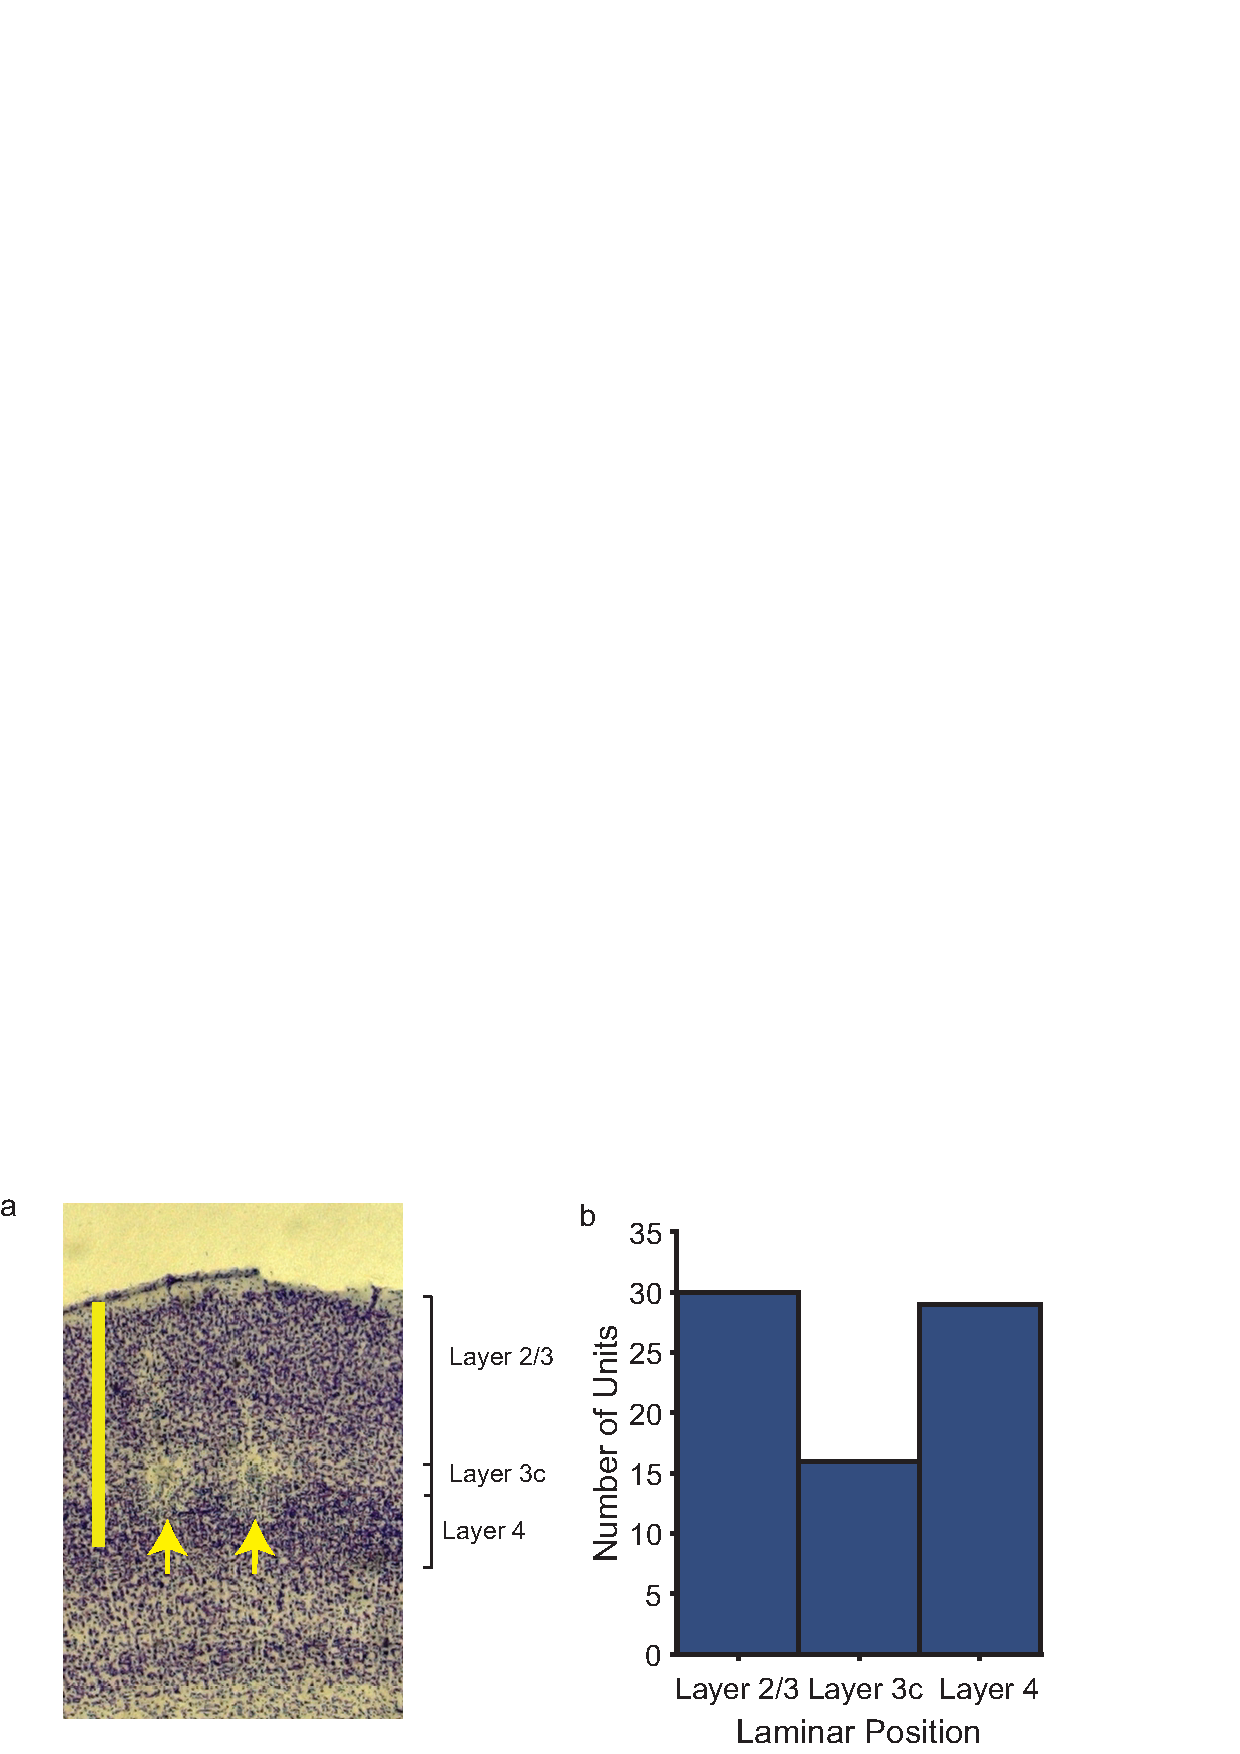
\includegraphics[width=\linewidth]{ShrewV1/LaminarPosition.jpg}
	\caption{The distribution of laminar positions from which we recorded. a) A photomicrograph of the tree shrew primary visual cortex with layers 2/3, 3c and 4 marked. The two arrows point to two lesions made in layer 3c of two separate tracks. The scale bar is 1 mm. b) Histogram showing the number of neurons recorded from each of the layers.}
	\label{fig:lp}
\end{figure} 


\subsubsection{Distribution of the circular variance}

The distribution of circular variances for neurons in the three layers,
calculated from their responses to thin moving bars are shown in fig 2.
The median CV of layer 2/3 neurons was 0.59 (n=28; 95\% CI= {[}0.32,
0.68{]}); that of layer 3c was 0.87 (n= 16; 95\% CI= {[}0.68, 0.91{]})
and that of layer 4 neurons was 0.88 (n=29; 95\% CI={[}0.84, 0.90 {]}).
The three distributions were significantly different from each other
(p\(<\)0.001, Kruskal-Wallis test). Post-hoc tests revealed that there
was a statistically significant distribution between the distribution of
CVs of neurons in layer 2/3 and layer 3c (Wilcoxon rank sum test,
z=2.37; p\(<\)0.01) and between layer 2/3 and layer 4 (Wilcoxon rank sum
test test, z= 3.58, p\(<\)0.001). The difference between the
distributions of CV of layer 3c neurons and layer 4 neurons was not
statistically significant (Wilcoxon rank sum test, z= 0.67; p=0.25).

\begin{figure}[H]
	
	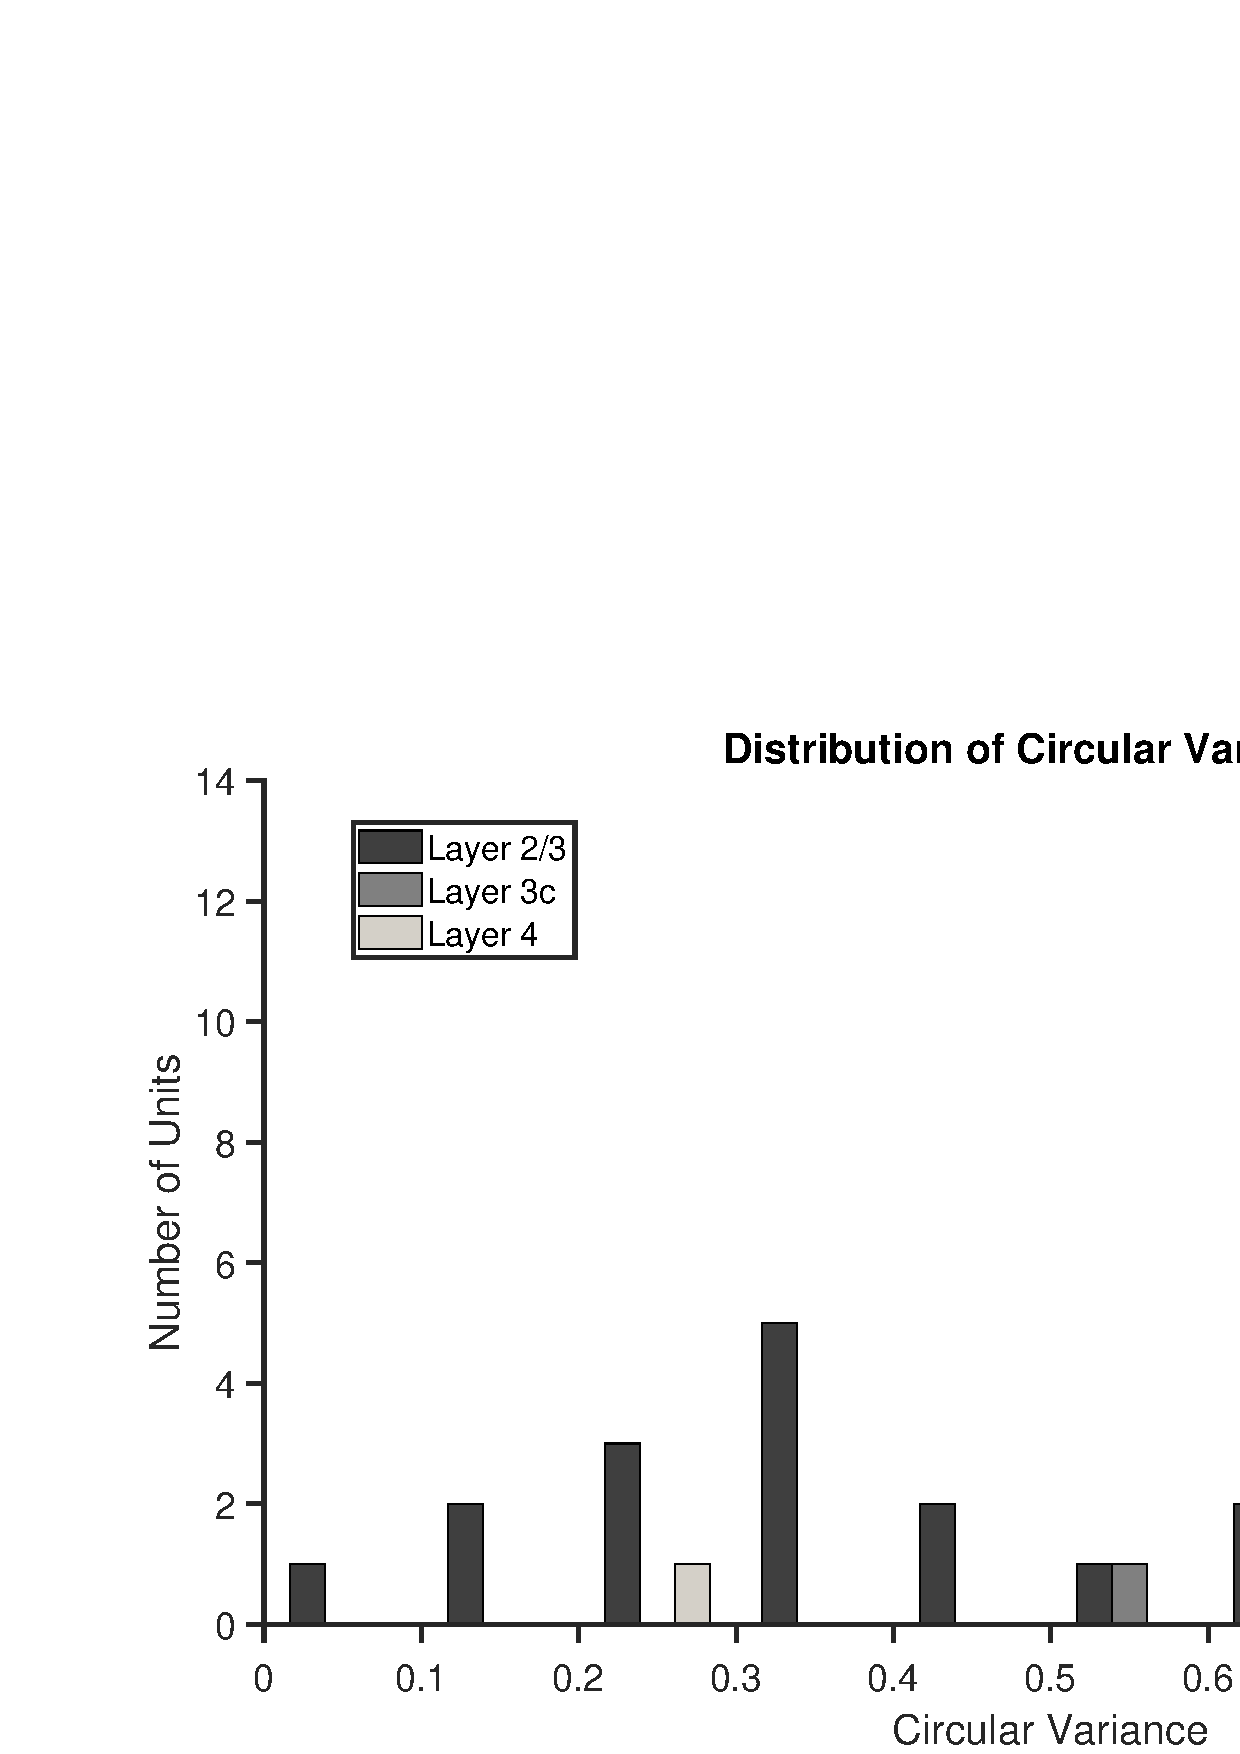
\includegraphics[width=\linewidth]{ShrewV1/cv_lamina_2_bw.jpg}
	\caption{The distribution of circular variance of neurons of the shrew V1.}
	\label{fig:cv}
\end{figure} 

\subsubsection{Circular mean of neurons}

In \textbf{{[}H1{]}}, we predicted that the layer 2/3 and layer 4
neurons in each track will have the same orientation. In this section,
we aimed to test this hypothesis. To test this hypothesis, we took the
absolute difference between the circular means of each layer 2/3 neuron
and all the layer 4 neurons from that track. Since layer 3c neurons
showed a similar degree of orientation selectivity as the layer 4
neurons and it has been shown that layer 3c also receive direct inputs
from the LGN (Reference), we also took the absolute difference of the
layer 3c neuron's orientation from the corresponding layer 2/3 neuron.
The results from 37 pairs of neurons from 18 tracks are presented in fig
3. We found that there were two peaks, one with the centre at
0\textsuperscript{o} and the other at 65\textsuperscript{o}. The
distribution of absolute differences was significantly different from a
uniform distribution (chi-square test; n=37; df=5; chi-square=12.35;
p\textless{}0.005).

	\begin{figure}[H]
	\centering
	\includegraphics[width=0.5\linewidth]{ShrewV1/cmdiff.jpg}
	\caption{The absolute difference between the circular mean of the first layer 2/3 neurons in each track and subsequent neurons from layer 3c and layer 4 in each track.}
	\label{fig:cmdiff}
\end{figure}


We then split the distribution into two groups: pairs of neurons that
were tuned to orientations less than 45\textsuperscript{o} (Group 1)
apart and pairs tuned to orientation greater than 45\textsuperscript{o}
apart (Group 2). We then determined if the absolute difference was
between the layer 2/3 neuron and layer 3c neurons or between layer 2/3
neuron and layer 4 neurons. These results are shown in fig.4. We found
that in Group 1, the majority of the difference pairs were between layer
2/3 and layer 4 neurons (N=15; Binomial Distribution, p=0.04). In Group
2, majority of the difference pairs were between layer 2/3 and layer 3c
neurons (N=22; Binomial Distribution, p=0.04)


\begin{figure}[H]
	\centering
	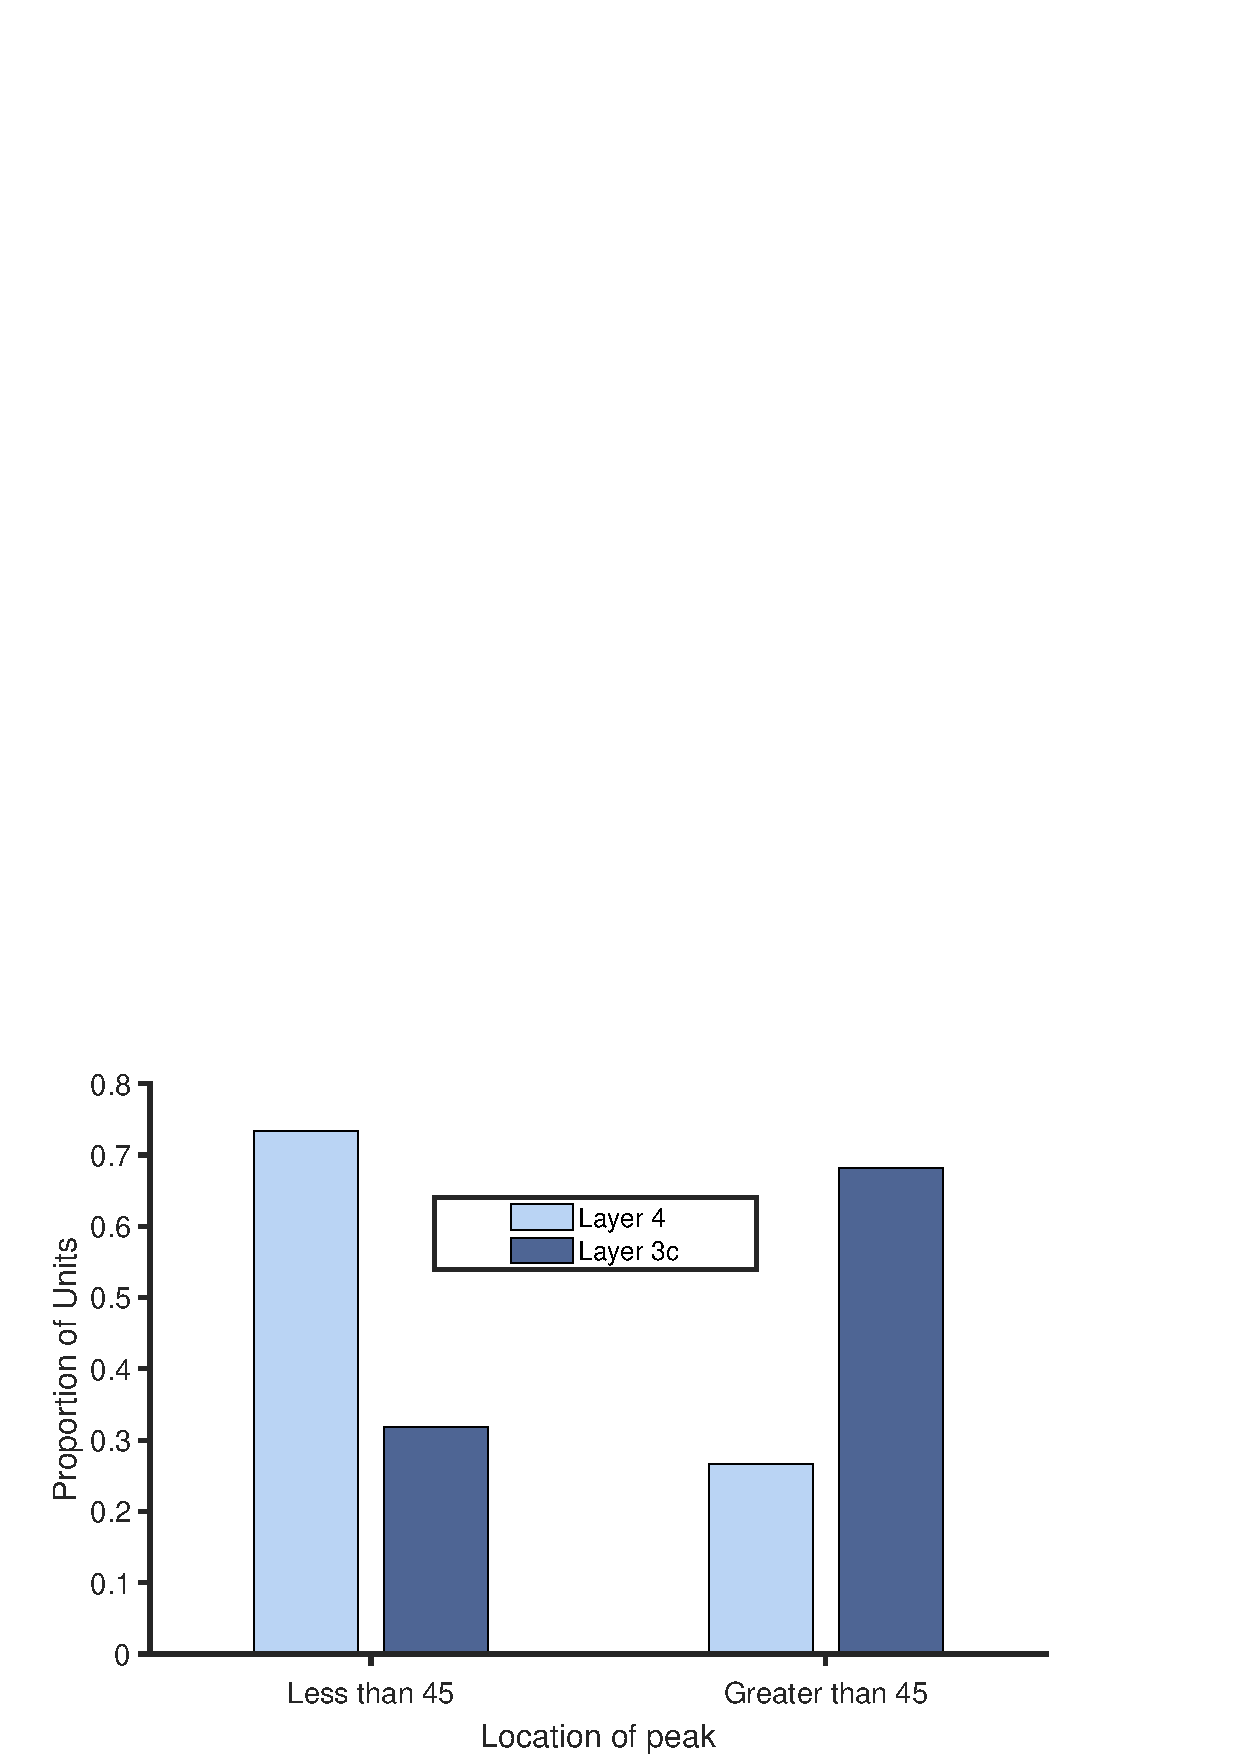
\includegraphics[width= 0.5\linewidth]{ShrewV1/cmlayer.jpg}
	\caption{The proportion of neurons from layers 3c and layer 4 with absolute differences greater and lesser than 45$^o$.}
	\label{fig:cmlayer}
\end{figure}

In order to ensure that the second peak we observed in fig. 4 wasn't due
to track angles, we undertook a simulation experiment (See methods
section). We found that for the shortest distance between the layer 2/3
and layer 4 neurons in our sample (50 mm), there was a high probability
of getting an absolute difference of 0 but this probability decreased
steadily. For the greatest horizontal distance between two neurons in
our sample (300 mm), the probability of obtaining the same orientation
was lower. While there was a general trend towards getting neurons that
were tuned closer to 90\textsuperscript{o} apart, there was no specific
bias for a difference of 65\textsuperscript{o}. The highest probability
of obtaining a peak at 65\textsuperscript{o} was when the horizontal
distance was 250 mm (p=0.045).

\begin{figure}[H]
	\centering
	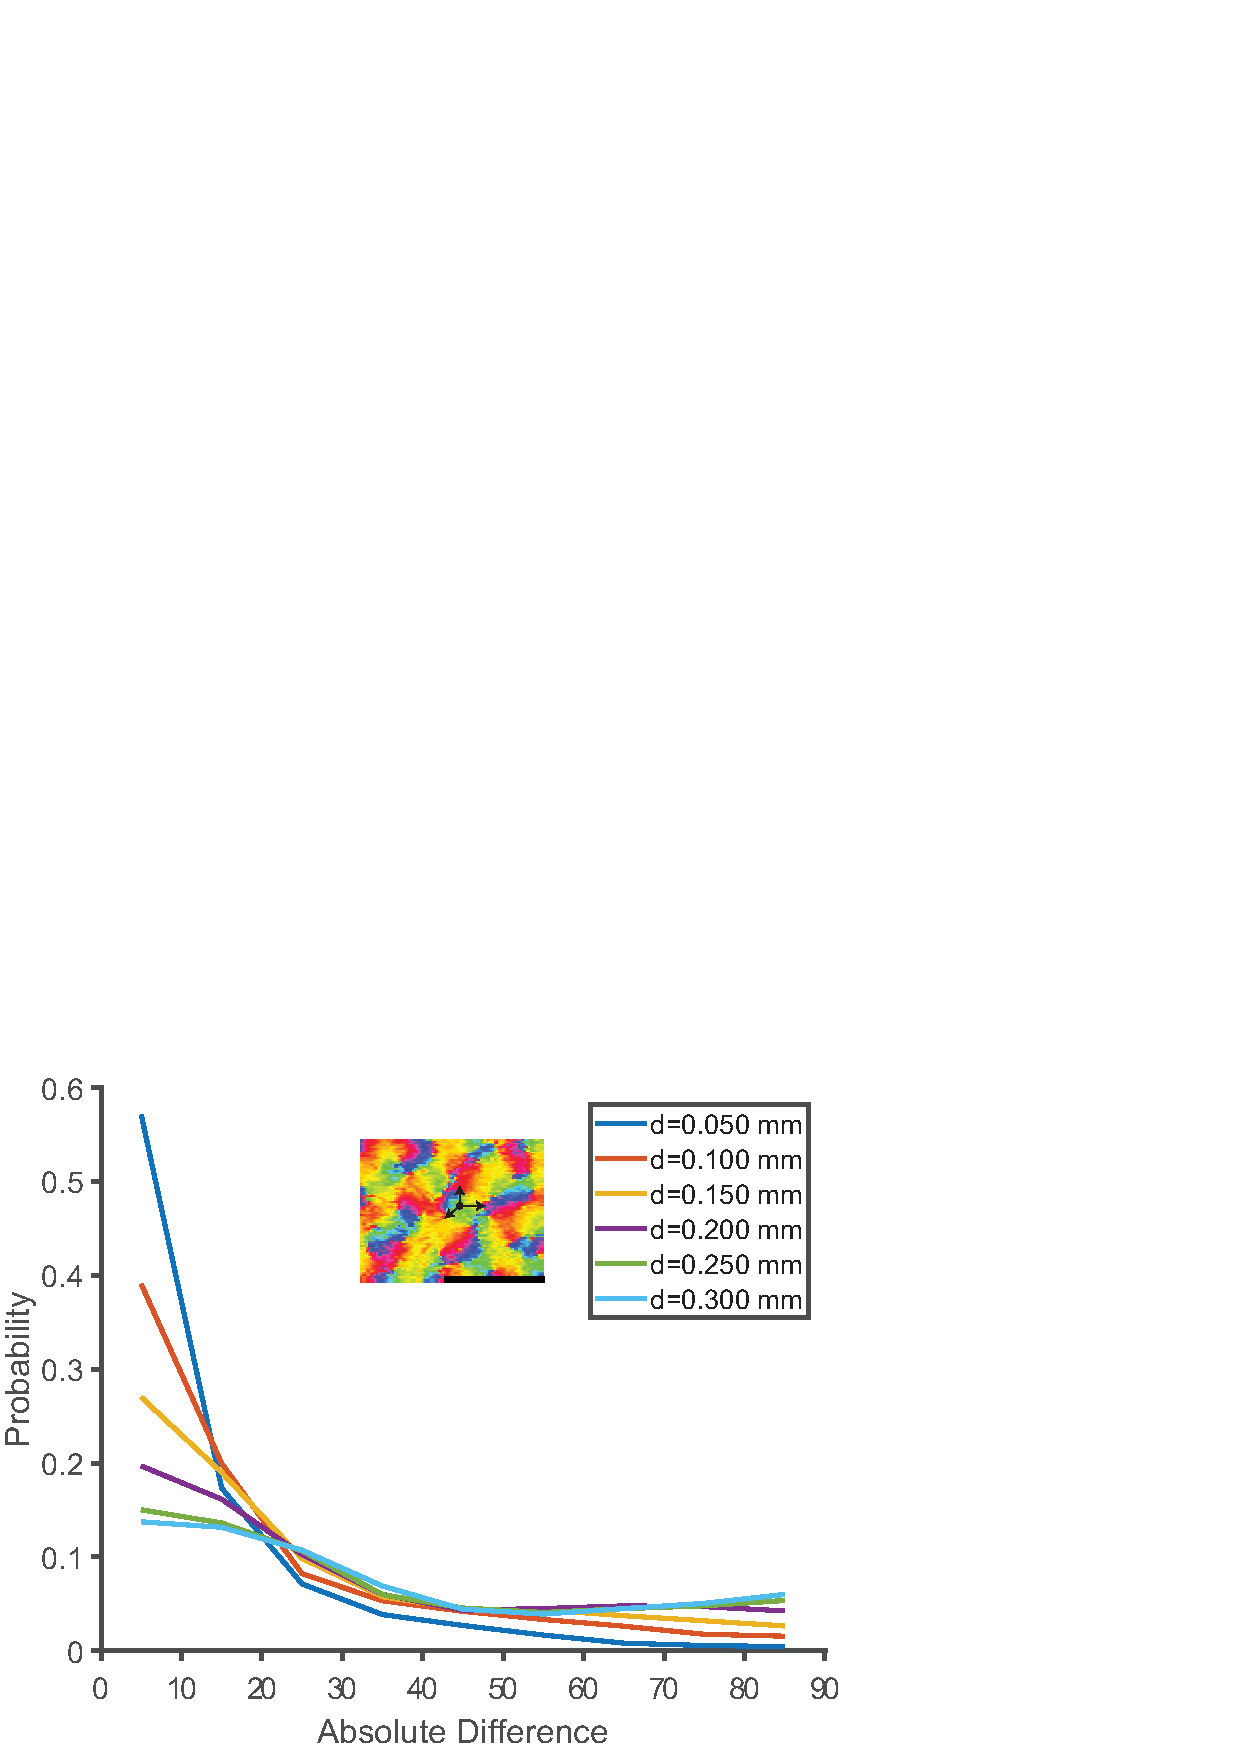
\includegraphics[width=0.6\linewidth]{ShrewV1/simulation.jpg}
	\caption{Results of a simulation experiment: The orientation tuning map (inset) was taken from Bosking et al., 1997. On this map, points were randomly placed and the orientation of 1000 pixels randomly selected at one of the distances in the legend was subtracted from the original data point. For each distance, the distribution of absolute differences for the 1000 pixels are shown by the lines in the graph. Black line is 1mm.}
	\label{fig:sim}
\end{figure}

\subsubsection{Spatial Frequency Tuning of neurons}

The distribution of the low cut-off, preferred and high cut-off spatial
frequencies of the neurons in layer 2/3 and layer 4 are shown in fig. 6.
Results from only these two layers are shown as we propose that the
orientation selectivity of layer 2/3 neurons arise predominantly from
layer 4 neurons. We found no significant differences between the spatial
frequency tuning between the two layers (n$_{23}$=27;
n$_{4}$=27; optimum spatial frequency: Wilcoxon rank sum,
z=-0.29, p=0.76; low cut-off: Wilcoxon rank sum, z=-0.75; p=0.45; high
cut-off: Wilcoxon rank sum, z=-1.69, p=0.09). although layer 2/3 neurons
tended to show high spatial frequency attenuation when compared to layer
4 neurons. When the bandwidth of spatial frequency tuning in octaves was
calculated, we found that the layer 2/3 neurons showed slightly sharper
tuning (median layer 2/3 b$_{oct}$= 2.2; n=16; median layer 4
b$_{oct}$=2.3; n=9). 11 of the 27 layer 2/3 neurons and 18 of
the 27 layer 4 neurons were low-pass tuned to spatial frequency.

		\begin{figure}[H]
	
	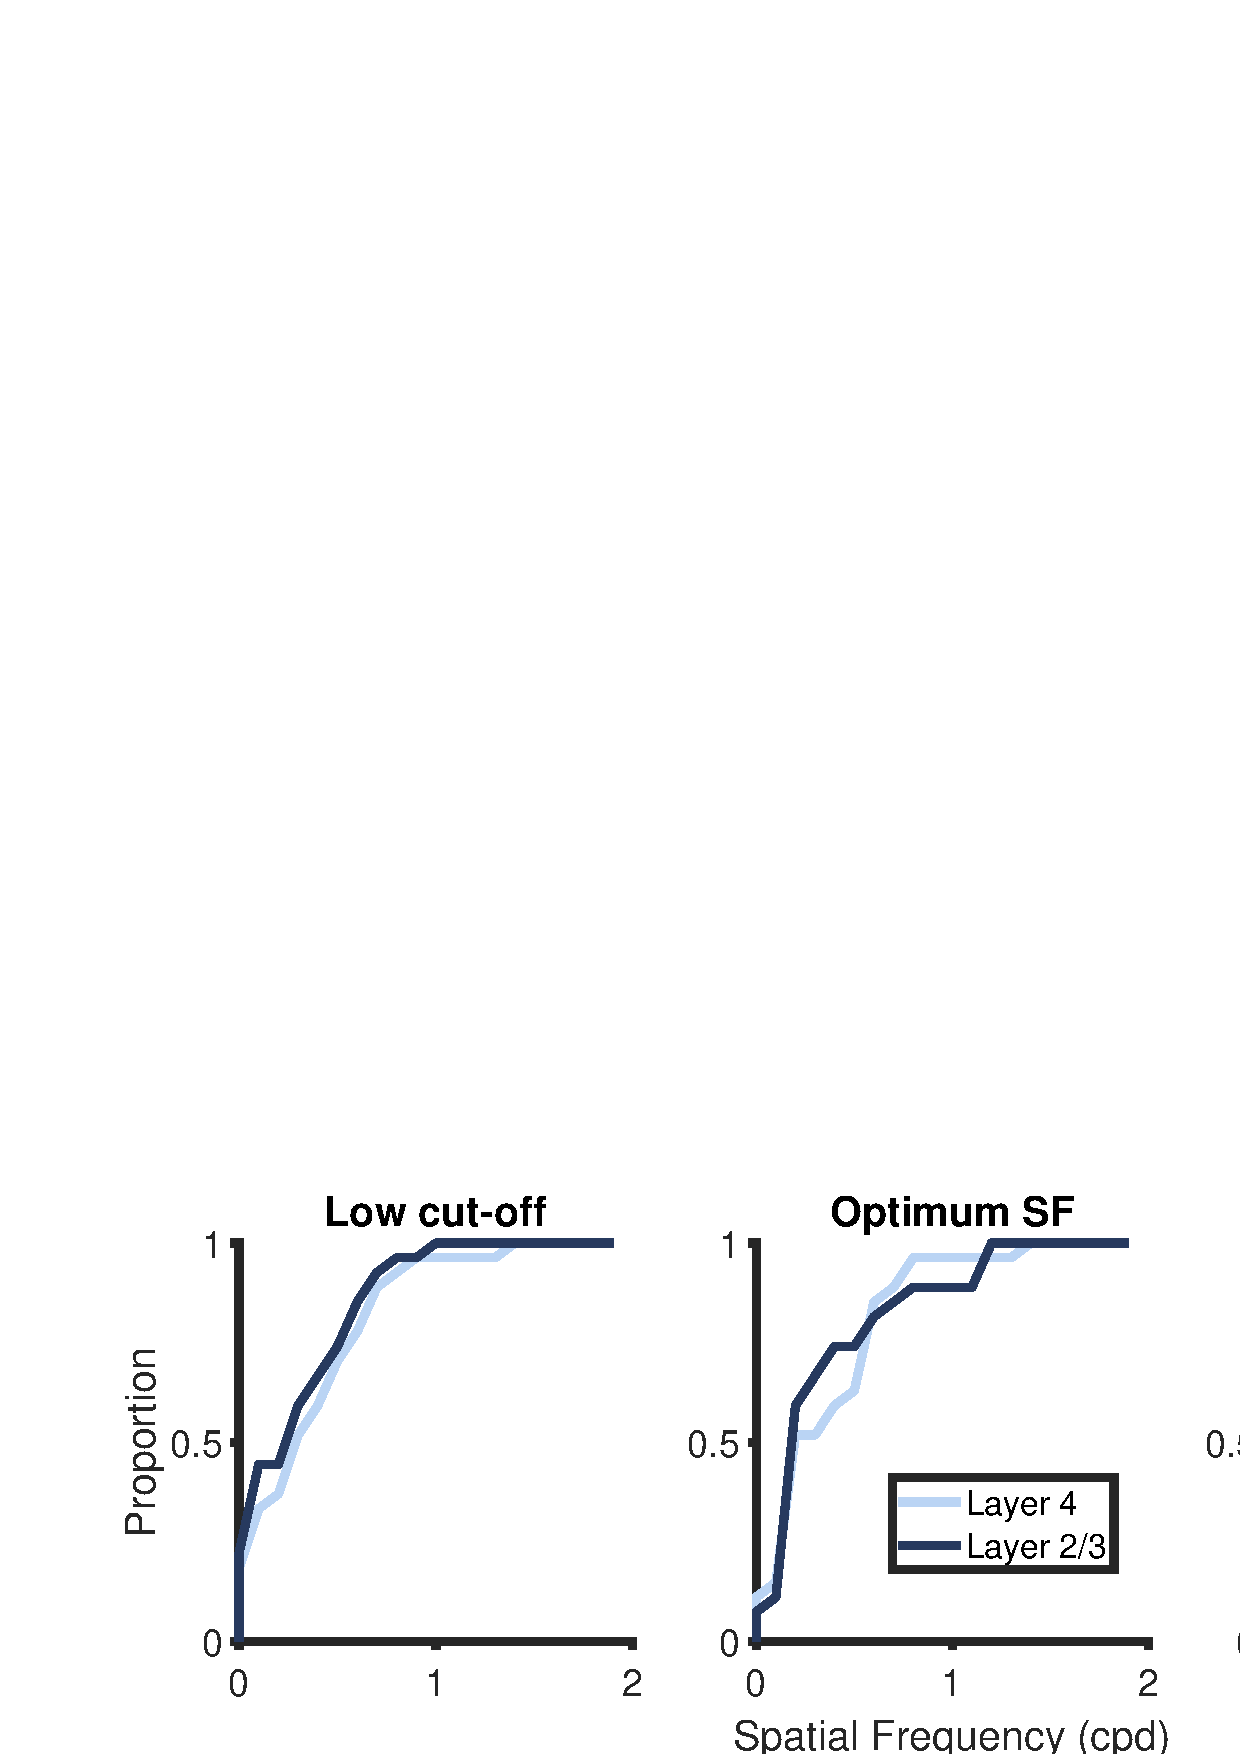
\includegraphics[width=\linewidth]{ShrewV1/sftuning_neurons_2.jpg}
	\caption{The cumulative distribution of the spatial frequency tuning of neurons in layers 2/3, 3c and 4 of the Shrew V1.}
	\label{fig:sftuning}
\end{figure}


In \textbf{[H2]}, we predicted that the layer 4 neurons will be more
tuned to orientation at higher spatial frequencies. We tested this
hypothesis by comparing the optimum spatial frequency tuning of layer 4
neurons with the spatial frequency where they demonstrated most
orientation tuning in 20 neurons. These results are presented in fig. 7.
Most neurons are located above the identity line, indicating that the
spatial frequency where they are maximally tuned for orietnation is
greater than the optimum spatial frequency of the neuron. The median
optimum spatial frequency of the layer 4 neurons was 0.35 cpd (95\% CI=
{[}0.2, 0.6{]}). The median of the spatial frequency where the
orientation selectivity index was the highest was 0.8 cpd (95\% CI=
{[}0.6, 1.2{]}). The spatial frequency at which the layer 4 neurons were
most tuned for orientation was significantly higher than the neurons'
optimum spatial frequency (Wilcoxon rank sum test, n=20, z= -2.93,
p\(<\)0.005).

\begin{figure}[H]
	
	\includegraphics[width=\linewidth]{ShrewV1/layer4OSI_highres.jpg}
	\caption{The relationship between the optimum spatial frequency of the layer 4 neurons and the spatial frequency at which the layer 4 showed the highest OSI. The dashed line is the identity line. The solid red line is the result of a linear fit of the form y=mx+c to the data (m= 0.73 [-0.15, 1.61] and c=0.58 [0.15, 1.01]). }
	\label{fig:OSI4}
\end{figure}


The results from 18 tracks where we compared the peak spatial frequency
of the layer 2/3 neurons and the spatial frequency where the layer 4
neurons were tuned for orientation are shown in fig.8. Fig 8a shows the
spatial frequency tuning curve of a layer 2/3 neuron and that of the
corresponding layer 4 neuron to the optimum and orthogonal orientation.
We hypothesised \textbf{{[}H3{]}} that the optimum spatial frequency of
the layer 2/3 neuron and the spatial frequency at which the layer 4
neurons was most tuned for orientation would be similar. We found that
this relation held true only in 3 of our 18 tracks. The median of the
optimum spatial frequencies of the layer 2/3 neurons was 0.2 cpd (95\%
CI= {[}0.1, 0.4{]}). In this sample of layer 4 neurons, the spatial
frequency where the neurons were most tuned to orientation was 0.8 cpd
(95\% CI= {[}0.3, 1.2{]}). In most of the tracks the maximum OSI of the
layer 4 neurons occured at higher spatial frequencies when compared to
the optimum spatial frequency of the layer 2/3 neuron (Wilcoxon signed
rank test, n=18, p\(<\)0.005) as demonstrated by the data points skewed
closer to the y-axis.

\begin{figure}[H]
	
	\includegraphics[width=\linewidth]{ShrewV1/sfsummary.jpg}
	\caption{The cumulative distribution of the spatial frequency tuning of neurons in layers 2/3, 3c and 4 of the Shrew V1.}
	\label{fig:sfsum}
\end{figure}



\section{Discussion}

In this chapter, we used extracellular recordings from layers 2/3 and
layer 4 of the tree shrew V1 to examine if orientation selectivity could
arise from sharpening the biased inputs from layer 4 neurons via the
ALD-RM model. As hypothesized, we found that the layer 4 neurons and the
layer 2/3 neurons were tuned to similar orientations \textbf{(H1)} and
that as the spatial frequency of the stimulus increased, the orientation
tuning of the layer 4 neurons got sharper \textbf{(H2).} In
\textbf{(H3)}, we hypothesised that the layer 2/3 neuron's peak spatial
frequency would be similar to the spatial frequency where the layer 4
neurons showed maximum orientation tuning. We found that this was only
true in three neuron pairs. These results are further discussed below.


\paragraph{Sharpening of orientation tuning in layer 2/3 and layer 4}

In this chapter, we determined the orientation selectivity of V1 neurons
from Layers 2/3, 3c and 4. We found that most neurons in layer 4 and
layer 3c were broadly tuned to orientation. While layer 2/3 neurons
showed sharper tuning to orientation overall, individual neurons showed
a bimodal distribution of orientation selectivity. These results are
consistent with previous results published in the tree shrews (Van
Hooser et al., 2013) and those published in the primary visual cortex of
macaques and cats where a wide range of orientation selectivities was
reported in V1 (Ringach et al., 2002).

In our study we used oriented bars to measure the degree of orientation
selectivity of neurons. Bars stimuli have a complex spatial frequency
spectrum and yield higher values of orientation selectivity when
compared to gratings of the optimum spatial frequencies (Reference). As
neurons showed better orientation selectivity to bars, it was easier for
us to determine the optimum orientation for further testing when bar
stimuli were used. However, it is likely that we have over-estimated the
extent of orientation selectivity, especially in layers 3c and 4 of
shrew V1. Van Hooser and colleagues also showed that there were two
groups of layer 4 neurons, those towards the edges of the layer 4 that
showed sharp orientation tuning and those in the middle that showed
broader orientation selectivity. In our sample (29 neurons), we only
found one layer 4 neuron that showed sharp orientation tuning, however,
this does not exclude the presence of more sharply tuned units at the
edges of layer 4.


\paragraph{Orientation columns in the tree shrew V1.}

In \textbf{H1}, we hypothesised that if the excitatory input from layer
4 neuron informed the orientation selectivity of the layer 2/3 neuron,
then both neurons will have the same optimum orientation. We found that
this was indeed the case. This also indicates that within an electrode
track, the columnar architecture observed in layer 2/3 might already be
present in layer 4. Surprisingly however, we found that layer 3c neurons
in V1 were tuned to an orientation 65\textsuperscript{o} away from the
optimum orientations of the layer 2/3 and the layer 4 neurons,
indicating that there is a laminar segregation in the optimum
orientation of neurons in the tree shrew V1. Neurons in this layer also
show broader orientation tuning unlike other layer 2 or 3 neurons. Here
we examine two possibilities for the difference in receptive field
properties of layer 3c neurons.

\textbf{Layer 3c is an input layer and is an extension of layer 4.}

The bottom of layer 3c neurons get inputs from layer 6 neurons in the
LGN in tree shrews. As a result, it has been suggested that this layer
might be an extension of layer 4, the LGN input layer in tree shrews
(Conley et al., 1984). Our results where the orientation biases of layer
3c neurons are similar to that of layer 4 neurons also supports this
hypothesis (also see Van Hooser et al., 2013). Further, it has also been
shown that while there are extensive horizontal connections within
layers 2-3b, layer 3c lacks horizontal connections, similar to layer 4.

\textbf{Layer 3c forms part of the koniocellular pathway in tree shrews.}

In macaques, layer 3B, which is located just above layer 4, contains
neurons that are broadly tuned to orientation. This layer receives
direct koniocellular inputs (from W-like cells) and shows blobs when
stained with cytochrome oxidase. As layer 3c cells receive inputs from
W-like cells, it has been suggested that layer 3c parallels layer 3b in
the tree shrew cortex. It is however important to note that it was layer
3b neurons and not layer 3c neurons in the tree shrew cortex that showed
patchy cytochrome oxidase staining. As a result, the pathway from W-like
cells in the retina via layer 3 of the LGN to layer 3B of V1 could be
the equivalent of the koniocellular pathway in macaques.

\textbf{Layer 3c provides cross orientation inhibition to layer 2/3 neurons.}

Another possibility could be that the neurons in layer 3c could be
providing inhibitory inputs to the layer 2/3 neurons. As we have shown
in this study, the layer 3c neurons show broader orientation selectivity
when compared to the rest of the layer 2/3 neurons and are tuned to an
orientation 65\textsuperscript{o} away from the orientation of the
corresponding layer 2/3 and layer 4 neurons. Layer 3c neurons are also
meant to receive inputs from the layer 4 (Fitzpatrick, 1996). Layer 3c
neurons could pool responses from the layer 4 neurons and provide the
basis for cross orientation inhibition in the layer 2/3 neurons rather
than both excitatory and inhibitory inputs arising from layer 4. If the
excitatory and inhibitory inputs from layer 4 and layer 3c neurons serve
to establish the initial orientation selectivity, then horizontal
connections in layer 2/3 could amplify the orientation response of the
neurons through recurrent excitation. This would also explain the
results of experiments where the stimulation of horizontal connections
had an additive effect rather than the modulatory effect previously
attributed to them (Huang et al., 2014).


\paragraph{Distribution of Spatial Frequency}

We also observed that spatial frequency tuning sharpened from layer 4 to
layer 2/3, however this sharpening was not statistically significant
(2.2 octaves to 2.3 octaves from layer 4 to layer 2/3). However,
bandwidth calculation could only be made in neurons that showed band
pass spatial frequency tuning. There was a significant change in the
number of layer 4 neurons that were low pass tuned to spatial frequency
(67\%) when compared to the layer 2/3 neurons (41\%). Of the bandpass
tuned neurons, layer 2/3 neurons also showed higher spatial frequency
attenuation. These results indicate that there was sharpening of
orientation selectivity from layer 4 to layer 2/3 in the tree shrew V1.

It is also important to note that when the low pass, optimum and high
pass spatial frequencies of neurons were compared, there was no
statistically significant differences between the three layers,
suggesting that the distribution of spatial frequency tuning stayed
similar throughout the primary visual cortex. Taken together with the
sharpening of spatial frequency tuning from layer 4 to layer 2/3
neurons, these results indicate that in most layer 2/3 neurons, there is
a direct sharpening of the inputs and the extensive low spatial
frequency attenuation reported in cats (Ref.) happens to a lesser extent
in tree shrews.


\paragraph{Spatial Frequency Dependence of Orientation Tuning}

We examined if the orientation selectivity of layer 4 neurons varied in
relation to the spatial frequency tuning of the neurons. We found that
in most cases, layer 4 neurons showed sharper orientation selectivity at
higher spatial frequencies as predicted in \textbf{(H2)}. In the tree
shrews then, orientation tuning of the layer 2/3 could be explained if
these neurons responded best at spatial frequencies where the layer 4
neurons were showed sharper orientation selectivity as suggested in
\textbf{(H3)}. However, when we tested \textbf{(H3)}, we found that it
was true only for a small proportion of neurons. In only 5 pairs of
neurons (out of 18) did the layer 2/3 neuron respond best at or above
the spatial frequency where the layer 4 neuron was best tuned to
orientation. In the other pairs, the layer 4 neurons were optimally
tuned for orientation at spatial frequencies higher than the optimum
spatial frequency of layer 2/3 neurons. What does it mean\ldots{}

In \textbf{(H3)} we hypothesised that the peak spatial frequency of the
layer 2/3 neurons would be similar to the spatial frequency where the
orientation tuning of the layer 4 neuron was greatest. We only found
this result in a small proportion of the neurons in our study. As a
result, while we cannot definitely conclude that neurons in layer 2/3
use non-specific inhibition to sharpen the orientation biases inherited
from the layer 4 neurons, we do have some evidence that suggests that
this could be the mechanism through which orientation arises in some
neurons in the tree shrew V1.
